% !TEX encoding = UTF-8 Unicode

\documentclass[twocolumn,10pt,a4j]{ltjsarticle}
\usepackage{kougai}
\title{楽曲のミックスダウンにおけるエフェクターによる\\効果と変化を理解するためのシミュレータ教材}
\author{1932148 依田 樹  指導教員 須田 宇宙 准教授}
\date{}

\begin{document}

\maketitle

\section{はじめに}
%背景
音楽制作には,メロディを作る「作曲」,歌詞を書く「作詞」,楽器の音を選択して伴奏を作る「編曲」などのほかに,複数の音源をエフェクターを用いて整え一つにする「ミックスダウン」という工程がある\cite{mix}.
近年はスマートフォンやタブレットでも手軽に音楽制作ができるようになった.また,近年のデジタル化により,機材がハードウェアからソフトウェアになり,ミックスダウンも費用をかけずに誰でも挑戦することができるようになった\cite{digital}.

%問題点
しかし,ミックスダウンは,作曲,作詞,編曲に比べ変化が分かりにくく非常に学びづらい.また,ミックスダウンの経験が少なく、エフェクターを使いこなせない人にとって、エフェクターの効果が説明だけではわからないという問題点がある.

%目的
そこで本研究では,実際に操作し,各エフェクターの使い方やその効果を知るためのシミュレータ教材を開発することを目的とする.

\section{楽曲のミックスダウンについて}
図\ref{fig:gainen}の左側にそれぞれの楽器の録音された音源があり,左から順番にエフェクターの効果を与え最終的にすべてをまとめて一つの楽曲の音源として完成させる.このような作業をミックスダウンという.
表\ref{table:effector}は,主にミックスダウンに使われるエフェクターをまとめたものである.

\begin{figure}[h]
\centering
 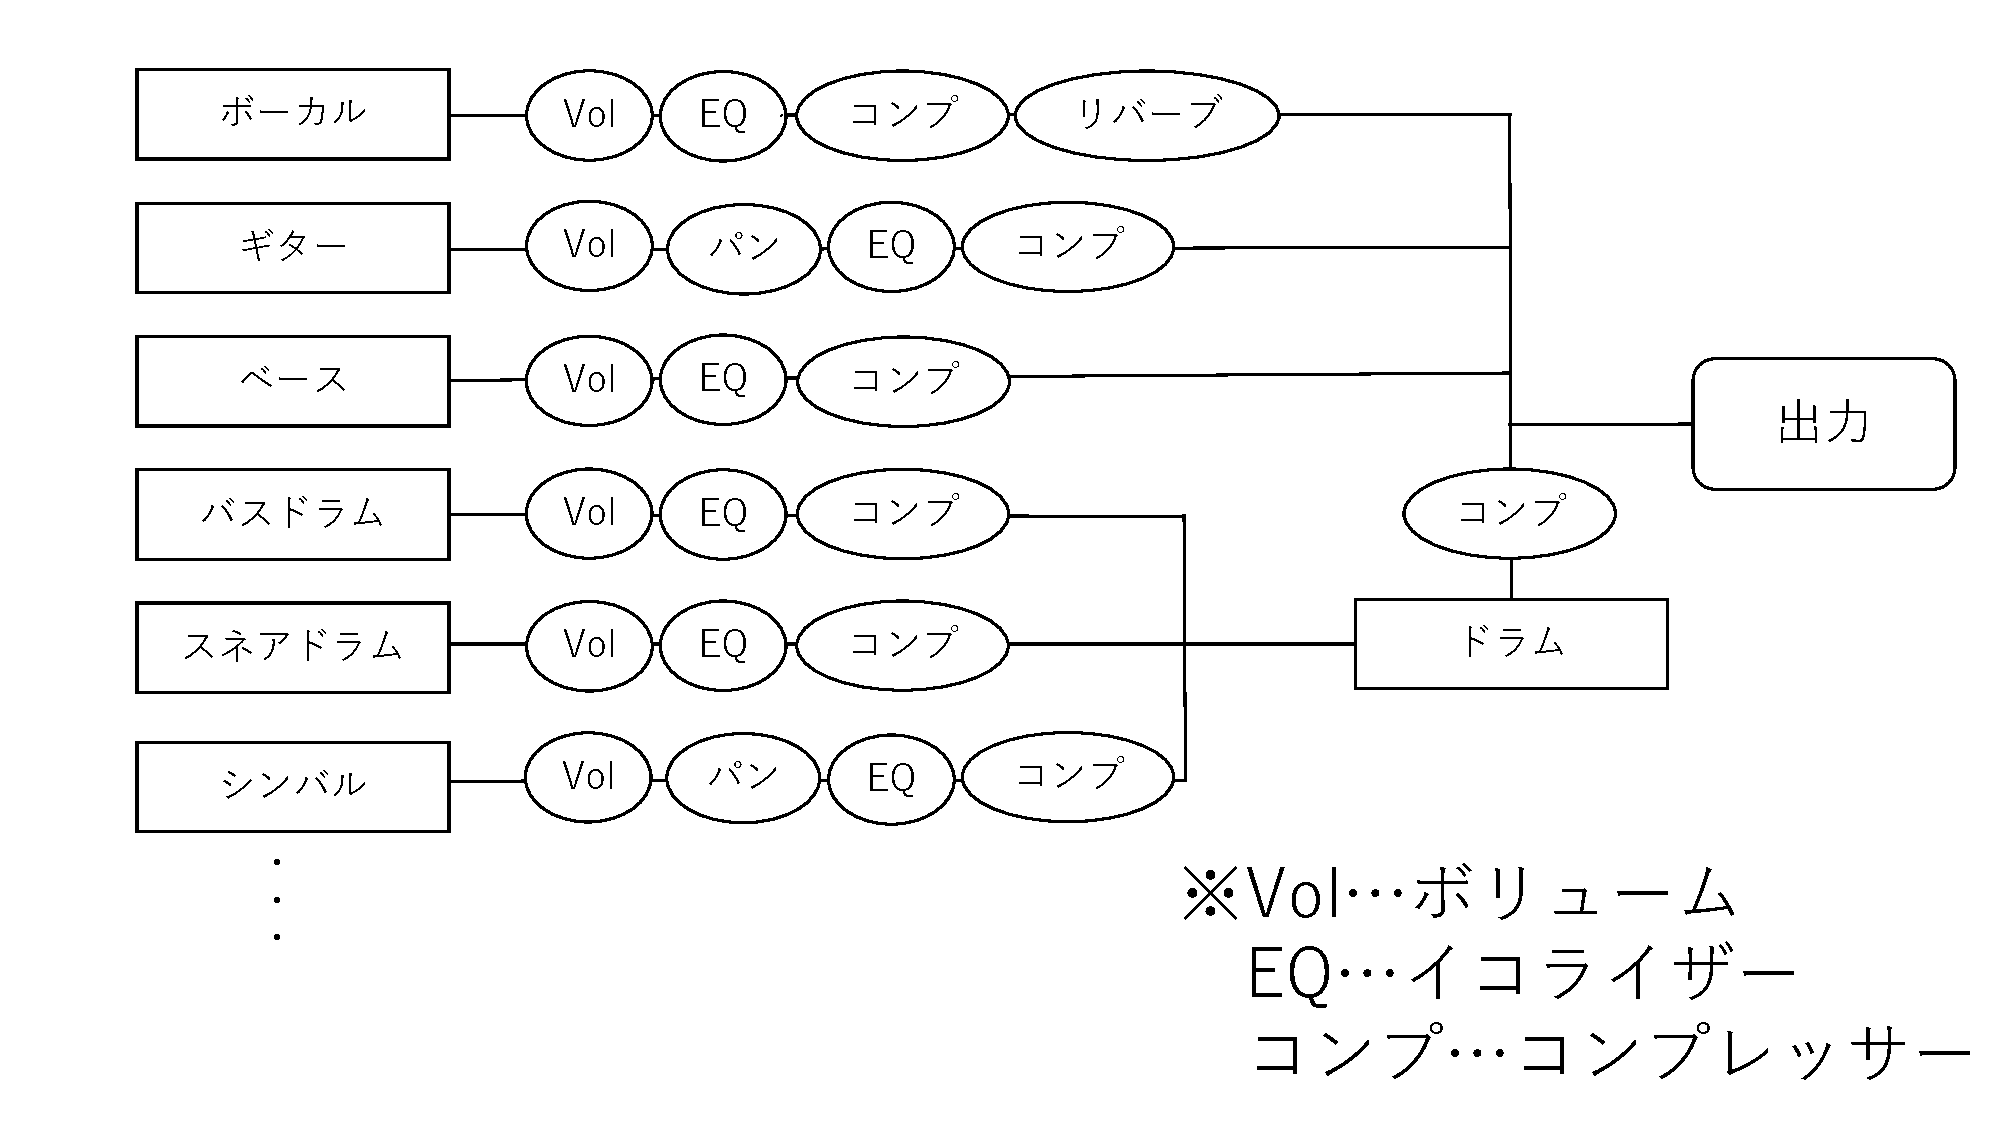
\includegraphics[width=85mm]{./figures/gainen.pdf}
 \caption{ミックスダウンの概念図}
 \label{fig:gainen}
\end{figure}

\begin{table}[h]
  \centering
  \caption{主なエフェクターとその効果}
  \label{table:effector}
  \small
  \begin{tabular}{cc}
    \hline
    エフェクター  & 説明    \\
    \hline \hline
    ボリューム  & 音源の音量調整 \\
    \hline
    パン  & 音源の左右位置の調整 \\
    \hline
    イコライザー  &  特定の周波数の音量調整 \\
    \hline
    コンプレッサー  &  音量の大小の幅を狭める調整 \\
    \hline
    リバーブ &  反響音の追加 \\
    \hline
    ディレイ  &  やまびこの効果を追加 \\
    \hline
  \end{tabular}
\end{table}

\section{シミュレータの構成}
学習者は,まず別ページの説明を読み,エフェクターについて学習する.
次に,エフェクターをオン・オフしたりパラメータを変更するなどして,エフェクターの効果を耳で理解する.
その後、ユーザーの持っている音源を読み込み,ユーザー自身がパラメーターを調整して,より理解を深めていくという流れを想定している.

シミュレータのレイアウトを図\ref{fig:layout}に示す.
\raise0.2ex\hbox{\textcircled{\scriptsize{1}}}は,音源を操作するためのコントローラーを表しており,それが縦に6つ並んでいる.
ボタンは左から,ファイルの読み込み,ミュート,単体再生,エフェクターの効果のオン・オフ,リセット,効果を与える音源の切り替え,となっていて,赤丸は,選択中の音源を表している.
\raise0.2ex\hbox{\textcircled{\scriptsize{2}}}のボタンは,音源の同時再生で,スライダーは,再生位置の調整となっている.
\raise0.2ex\hbox{\textcircled{\scriptsize{3}}}は選択中の音源のエフェクターの効果の掛かり具合のパラメーターを調整するスライダーとなっている.
\raise0.2ex\hbox{\textcircled{\scriptsize{4}}}は,選択中の音源のエフェクターの効果を可視化する図や音声波形などを表示している.

\begin{figure}[h]
\centering
 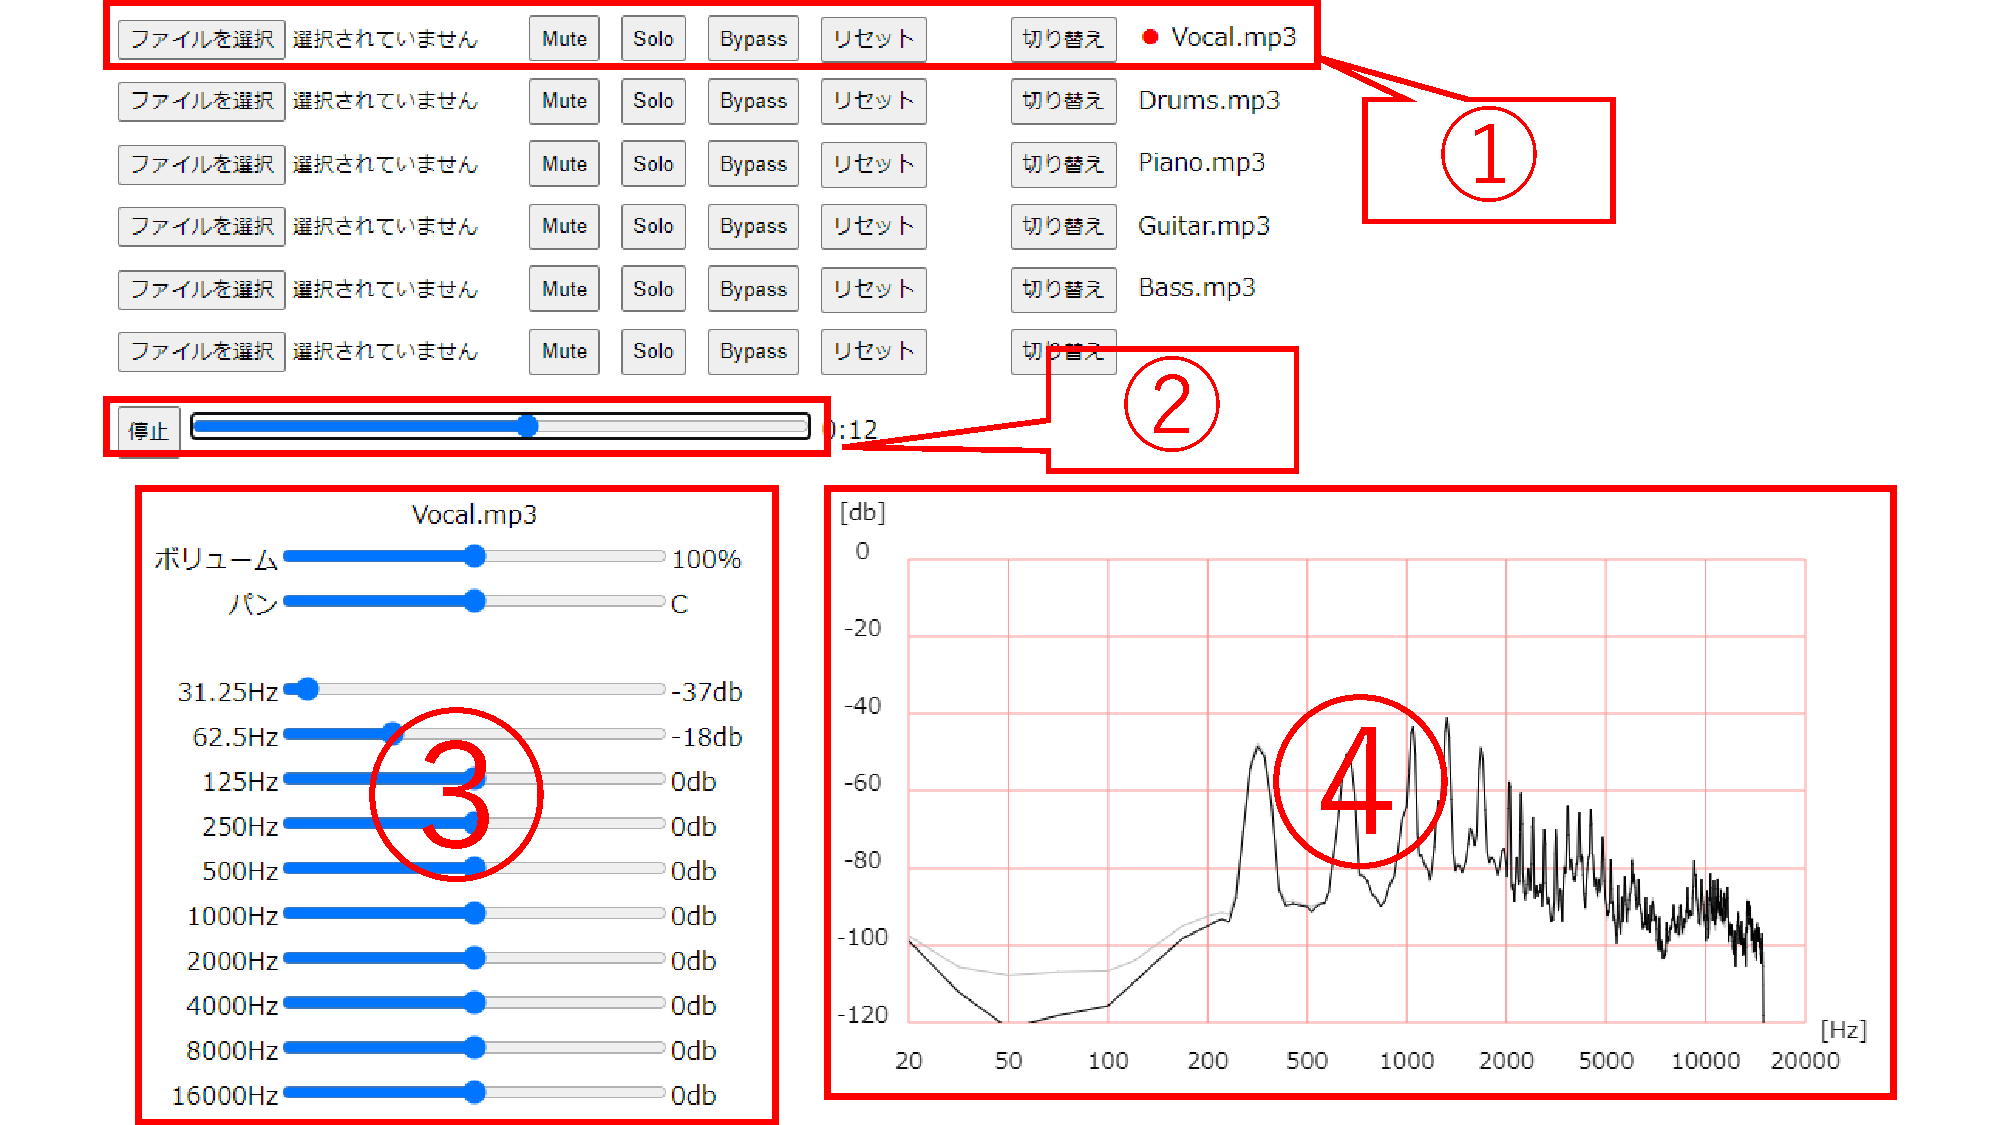
\includegraphics[width=85mm]{./figures/layout.pdf}
 \caption{開発したシミュレータ教材のレイアウト}
 \label{fig:layout}
\end{figure}

\section{おわりに}
本研究では,ミックスダウンにおけるエフェクターによる効果と変化を理解するためのシミュレータ教材を制作した.このシミュレータを使い、実際に体感することで、エフェクターへの理解が可能となることが期待される.

\begin{thebibliography}{99}
\bibitem{mix} ミックスダウンとは?その目的と作業内容、マスタリングとの違いを解説! \UTF{2013} OTO$\times$NOMA, \url{https://kensukeinage.com/whats_mix/}, 2022/8/21参照
\bibitem{digital} CDの「デジタル・リマスタリング」ってなんだ?|テクの雑学|TDK Techno Magazine, \url{https://www.tdk.com/ja/tech-mag/knowledge/062}, 2022/8/21参照
\end{thebibliography}

\end{document}
